
\chapter{Introduction}

\pagenumbering{arabic}


% {\bf need some more investigation to get the details right here}

Our view of the Cosmos changed dramatically during the first third of the XX century. The idea of a deterministic, stationary Universe governed by Newtonian dynamics with absolute measures of time and space had to be left behind as Quantum Mechanics and the Special and General Theories of Relativity revolutionized our understanding of the very small, the very fast and the very large, respectively, along with our notions of space and time themselves.

It was not long until astronomical observations came to revolutionize our understanding of the Universe just a little more and, with that, our very own place in it.
%
The year 1920 was host to one of the most famous astronomical discussions ever to take place. In what was termed ``the Great Debate,'' Harlow Shapley and Heber D.\ Curtis discussed (among other topics) the extent of the Milky Way and its place in the Universe (\citealt{shapley21}; a thorough review of the debate and its context is presented by \citealt{trimble95}). Shapley argued that the Milky Way, with a size of up to 100 kpc, composed the entire Universe, while Curtis argued that other ``spiral nebulae'' were distinct galaxies much like our own Milky Way (which, he argued, was much smaller and hosted the Sun in its very centre). The issue was settled not long after, thanks to the observation of Cepheid variable stars in the Andromeda nebula by \cite{hubble25}. It was already known at that time that a Cepheid's distance can be inferred by measuring the duration of its variability cycle, since they follow a tight period-luminosity relation. While Shapley was right that the Sun is not located at the centre of the Milky Way, Curtis was right about the nebulae: Hubble's observations were definitive proof that these spiral nebulae could not be part of our Galaxy, and marked the birth of \emph{extragalactic} astronomy. 

A few years later, \cite{hubble29} showed that there exists a linear relation between the distance and the velocity of galaxies other than the Milky Way (now known as Hubble's law), which became the first solid evidence for an expanding Universe. He based this inference on measurements of i) the period of Cepheid stars (from which he inferred their luminosities and thereby their distances) and ii) the Doppler shift of their spectra, using spectroscopic observations made by Vesto Slipher. A thorough discussion of pre-1929 observations of receding galaxies and discussions of an expanding Universe is presented by \cite{trimble12,trimble13}.

Then, in 1933 Fritz Zwicky showed that galaxies in galaxy clusters move faster than the sum of their masses would be able to hold gravitationally, and inferred that there must be 10 to 100 times more mass hidden from us. Zwicky's observations are now credited as the discovery of dark matter \citep[e.g.,][]{trimble87,einasto13}.

Our modern standard model of cosmology came to be complete with three additional ingredients: the discovery of the cosmic microwave background (CMB) by \cite{penzias65}, predicted by the hot big bang hypothesis \citep{dicke65}; the development of inflationary theory, which explains the homogeneity of the CMB with a brief period of exponential growth in the very early Universe \citep{guth81}; and the discovery of the Universe's accelerated expansion \citep{riess98,perlmutter99}. We use the term `dark energy' to refer to the cause of this accelerated expansion, whatever it may be. Dark energy makes up approximately 70\% of the energy density of the Universe, while dark matter amounts to about 25\%. Consequently, only about 5\% of the Universe corresponds to `normal' luminous matter \citep{planck15xiii}.
%Within this model, our current best estimate for the age of the Universe is about 14.3 Gyr \citep{planck15xiii}.


\section{Galaxy clusters}

\begin{figure}
 \centerline{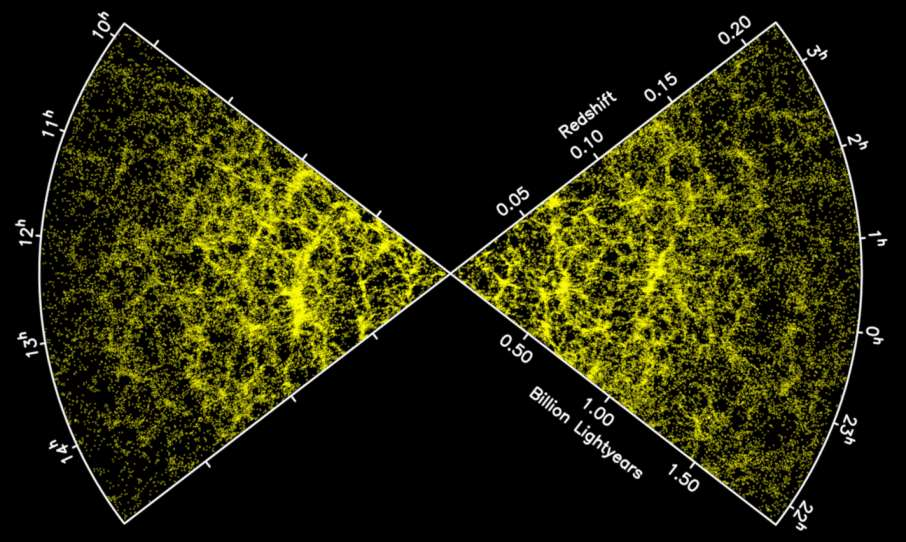
\includegraphics[width=4in]{chapter1/web_2df.jpg}}
\caption{The local ($z<0.2$) cosmic web as seen by the 2-degree-Field Redshift Survey. Each yellow dot is a galaxy with a spectroscopic redshift.}
\label{f:intro_web}
\end{figure}

% As introduced above, galaxy clusters gave the first clues of the existence of dark matter, and have 

The cosmological model introduced above predicts that structure grows hierarchically: small structures form first and then merge to give rise to larger structures. This continuous mass accretion and merging process has given rise to what we term the `Cosmic Web'; \Cref{f:intro_web} shows the local ($z<0.2$) cosmic web as seen by the 2-degree Field Redshift survey \citep{colless01}. At the intersections of this web lie galaxy clusters, the most massive structures formed so far in the Universe.

%Galaxy clusters are at the top of this hierarchy; being the most massive structures, they are also the latest to have formed.
As their name suggests, galaxy clusters are objects in which galaxies abound---a massive cluster can host hundreds of bright galaxies \citep[e.g.,][]{abell58}. However, this simple description was rendered insufficient early on by \citeauthor{zwicky33} (\citeyear{zwicky33}, discussed above). We now know that galaxy clusters, with sizes of 1$-$2 Mpc (with $1\,{\rm Mpc}=3.26$ million light-years) and masses of up to a few times $10^{15}\,\Msun$, are mostly made of dark matter (roughly 80\% of their mass); only about 2\% of their mass is in stars, while the remaining 18\% is in a hot ionized gas with temperatures exceeding $10^7$ K that can be observed at X-ray wavelengths \citep[e.g.,][]{sarazin86}.

\subsection{A look at their components}

Given their composition, galaxy clusters serve as unique laboratories to study the connection between light and mass in the Universe. The galaxies we readily see tell us the story of a harsh, unforgiving environment: unlike the spiral galaxies (or `nebulae') known since time immemorial (but only characterized over the course of the past century), galaxies in clusters are typically of elliptical shape and a distinct reddish colour \citep{dressler80,gladders00}. This difference arises because galaxies entering clusters suffer the fast removal of their cold ($\sim10$ K) gas (which can collapse to form stars); the galaxies are then left only with old stars, which on average look redder than young stars, which look bluer (hence the colour of spiral galaxies). 

Modern X-ray observatories, in turn, reveal the structure of the hot gas in great detail. The enormous gravitational potentials of clusters induce massive cooling flows which produce bursts of star formation in the cluster centres \citep[e.g.,][]{mcdonald12}, but such flows are easily disrupted by accreting supermassive black holes \citep[which are common in galaxies in the centres of clusters; e.g.,][]{?}, and by cluster-cluster collisions (also referred to as cluster mergers), which shock-heat the cluster gas \citep{?}. Cluster mergers (along with supernovae) produce some of the most spectacular X-ray images in the sky \citep[e.g.,][]{markevitch02,menanteau12}.

The third component, dark matter, can be studied with gravitational lensing: because mass curves space, the light from background galaxies is deflected as it passes near a mass overdensity on its way to our telescopes. This produces a coherent distortion of the observed shapes of background galaxies around any given cluster \citep{?}. One of the most compelling pieces of evidence for the existence of dark matter comes from the observation that the total mass distribution measured from gravitational lensing need not follow the luminous mass seen in the X-rays \citep[e.g.,][]{clowe06,dawson12}. Indeed, gravitational lensing studies have revealed that the dark matter in clusters can also follow wild distributions, all the way from a ring in the cluster CL J0024+17 \citep{jee07} to a veritable `train wreck' in Abell 520 \citep{jee14}.

% We can learn much more by combining observations of the different components...


\subsection{Mass proxies and cosmological leverage}

Galaxy clusters also reveal the ability of the Universe to aggregate matter: given the amount of matter in the Universe (and the speed of its expansion), there can only be so many clusters formed at a given time. Therefore galaxy clusters have the ability to constrain up to three cosmological parameters: the matter density, $\Omega_{\rm m}$, the amplitude of initial density fluctuations, $\sigma_8$, and the dark energy density, $\Omega_\Lambda$.

Exploiting clusters as cosmological probes requires knowledge of their masses, which is not an easy quantity to estimate. While gravitational lensing provides a direct measurement of the surface mass density (which can be deprojected into a total mass under some assumptions), it has not been generally available for large samples of clusters.

Because of this, considerable effort has been devoted to characterize a variety of mass \emph{proxies}---observable quantities that, we hope, depend on mass in as simple a manner as possible, but also that are readily measurable with current capabilities. The most obvious of these is the number of galaxies, usually referred to as `richness', which has received considerable attention in recent years. Although initial attempts found that the richness was a very noisy mass proxy, recent studies have found that a properly-defined richness can be as good a proxy as any other \citep{rykoff12,andreon15}. Also common are X-ray--derived mass proxies, including the X-ray luminosity, the gas temperature and the gas mass. Of these, the gas mass shows the least scatter \citep{mahdavi13} but is the most difficult to obtain, and is currently only available for rather small samples.

A novel mass proxy, which has only been measurable in recent years thanks to new sensitive, high-resolution millimeter-wave surveys is the Sunyaev-Zel'dovich \citep[SZ,][]{sunyaev72} effect. The SZ effect is the inverse Compton scattering of CMB photons as they interact with the hot electrons in galaxy clusters. In a sense, therefore, observing the SZ effect is like seeing the shadow of a galaxy cluster. Because it is a CMB observable, the SZ surface brightness is independent of the redshift of the cluster producing it, and SZ surveys reveal the most massive clusters at all redshifts \citep{hasselfield13,bleem15}.\footnote{This is not true for the SZ survey carried out with the \planck\ satellite, which is mostly limited to $z<0.6$ \citep{planck15xxvii}. This is because high-redshift clusters have a small angular extent, so their SZ signal is diluted by the large beam of \planck\ (roughly $5'$).} In contrast, X-ray or optical surveys are subject to the usual cosmological dimming of the surface brightness, $(1+z)^{-4}$, and are therefore generally limited to rather low redshift. In addition, the relation between SZ effect and mass has been predicted to have very little scatter \citep[at a level of 5--10\%; e.g.,][]{motl05,battaglia12}, although observations have shown that these predictions were rather optimistic \citep{benson13,sifon13}. In \citechapter{2} we characterize a newly discovered SZ-selected cluster at moderate redshift.

\begin{figure}
 \centerline{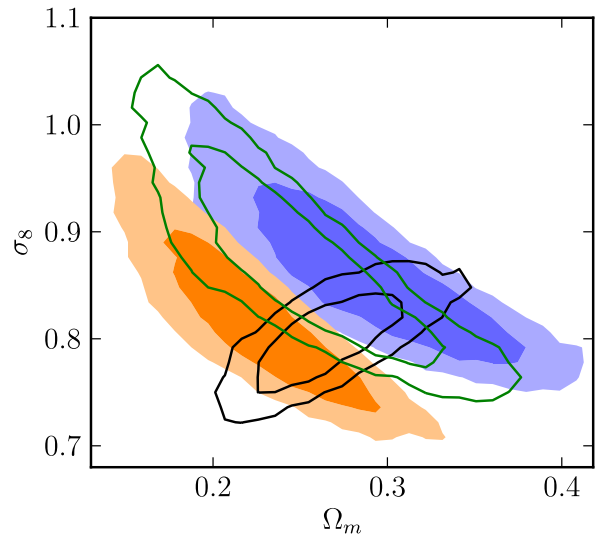
\includegraphics[height=2in]{chapter1/cosmo_SZ_ACT.png}
             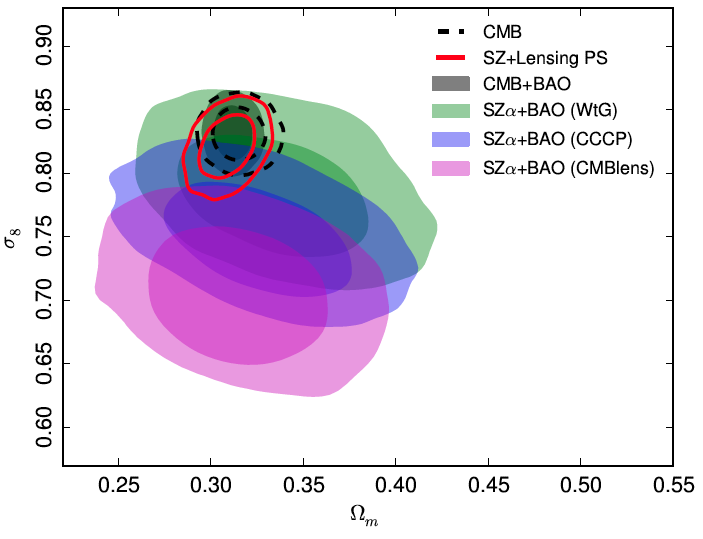
\includegraphics[height=2in]{chapter1/cosmo_SZ_Planck.png}}
\caption{Constraints on cosmological parameters $\Omega_{\rm m}$ and $\sigma_8$ from galaxy clusters detected by the Atacama Cosmology Telescope \citep[left, from][]{hasselfield13} and the \planck\ satellite \citep[right, from][]{planck15xxiv} through their SZ effect. Black contours in the left and right panel show constraints from primary CMB measurements by the WMAP and \planck\ satellites, respectively. The broader, coloured contours show different assumptions about the scaling between SZ effect and mass. Clearly, this dominates the uncertainty budget on cosmological parameters.}
\label{f:intro_szcosmo}
\end{figure}

Massive galaxy clusters at high redshift have a particularly strong leverage on cosmological parameters \citep{vikhlinin09}, so SZ surveys are particularly well-suited for cosmological parameter inference. The characterization of its properties as a mass proxy is an active field of study; this is the aim of \citechapter{3} in this thesis.
%
\Cref{f:intro_szcosmo} shows the constraints on cosmological parameters from galaxy clusters detected in the SZ survey by the Atacama Cosmology Telescope (ACT) \citep{hasselfield13} and the \planck\ satellite \citep{planck15xxiv}. Both analyses found that the main limitation to the constraining power is given by the unknown conversion from SZ effect to cluster mass, even though the ACT analysis is based on only 15 clusters.


\section{Cluster galaxies and subhaloes}

It was mentioned above that galaxies are drastically affected by their environment. In general, isolated galaxies are actively forming stars and have a disk-dominated morphology. However, upon being accreted by a galaxy cluster, they rapidly lose their cold gas (and thereby their ability to form new stars) due mainly to three effects, which can be briefly described as follows. `Galaxy harrassment' is the process by which a galaxy removes the gas from another galaxy due to a high-speed encounter or fly-by \citep{?}. `Ram pressure stripping' is the removal of galactic gas by the gas in the intracluster medium, because the galaxy is traversing it at high speed. Finally, `strangulation' refers to the process by which the gravitational potential of the cluster removes the cold gas from the galaxy due to the strong tidal forces.

The combined effect of these forces is most readily seen as a change in the colour and the morphology of galaxies, but there are other effects which have not been so well studied. Because galaxies and larger structures form by accretion of matter through the cosmic web, we expect them to point preferentially towards other mass concentrations in it. Indeed, observations show that this is the case for \emph{central} galaxies, but only the red or elliptical ones \citep{?}. These are mostly the galaxies in the centres of clusters and massive groups---the \emph{knots} of the cosmic web. Spiral or blue galaxies, which live in much less-dense regions, do not show such alignment \citep{?}. One of the outstanding questions, relevant to both galaxy formation models and measurements of weak lensing by the large-scale structure (`cosmic shear'), is whether the cluster potentials also align (or maintain the algnment of) their satellite galaxies; this is the question we address in \citechapter{4}.

Another aspect is the effect of the cluster environment on the dark matter content of infalling galaxies. %This is a difficult question to address even from numerical simulations, because of the difficulty in identifying dark matter subhaloes consistently in the first place.




\section{This thesis}

In this thesis we use a variety of observations and techniques to study the connection between the mass and light contents of galaxy clusters from different perspectives. This connection has implications

In \citechapter{2} we characterize \plck, a galaxy cluster recently discovered by the \planck\ satellite through its SZ effect. We present the first optical images of this cluster, measure its redshift ($z=0.52$) and identify multiple images of a background galaxy, which allows us to perform a strong lensing analysis. We also show that \plck\ hosts diffuse radio emission---the tell-tale sign of cluster mergers, and a still an extremely rare sight at $z>0.4$.

In \citechapter{3} we use extensive spectroscopic observations of galaxy clusters detected through the Sunyaev-Zel'dovich effect to measure the velocity dispersions of their member galaxies. Taking previous results from hydrodynamical simulations, we convert these velocity dispersions into cluster masses and compare them to the strength of the SZ effect, with the aim of characterizing the latter to allow its use for cosmological parameter inference. We pay particular attention to sources of uncertainty and scatter in the determination of the velocity dispersions, and conclude that the dominating uncertainty comes from the identification of member galaxies, which poses an irreducible uncertainty on velocity dispersions as mass proxies.

In \citechapter{4} we turn our attention to galaxies in clusters. We base our study on a sample of 90 clusters with deep, wide-field observations devised for accurate weak lensing measurements. After performing a thorough literature search for spectroscopic redshifts with which to select galaxies physically belonging to these clusters, we measure the orientations of cluster galaxies to see if there are any signs of alignment of galaxies within clusters.

In \citechapter{5} we take advantage of the overlap between the spectroscopic Galaxy And Mass Assembly Survey with the photometric Kilo-Degree Survey to measure the masses of satellite galaxies in galaxy groups using weak gravitational lensing, with the aim of constraining the segregation of group galaxies by mass. The spectroscopic nature of the galaxy group catalogue ensures we can do this essentially free of contamination from both non-group galaxies and central galaxies.

Finally, in \citechapter{6} we extend the lensing measurements of \citechapter{5} to more massive galaxy clusters using the dataset produced for \citechapter{4}. Using weak lensing measurements of the masses of cluster galaxies, we constrain the stellar-to-subhalo mass relation and again study the mass segregation of cluster galaxies.


% \begin{thebibliography}{}
% 
%  \bibitem[Dicke et al.(1965)]{dicke65} 
%  \bibitem[Einasto(2013)]{einasto13} Einasto, J., 2013, \bjp, 43, 369
%  \bibitem[Hubble(1929)]{hubble29} Hubble, E., 1929, \pnas, 15, 168
%  \bibitem[Planck Collaboration(2016)]{pcp15} Planck Collaboration, 2016, arXiv:1502.01589
%  \bibitem[Trimble(1987)]{trimble87} Trimble, V., 1987, \araa, 25, 425
%  \bibitem[Trimble(1995)]{trimble95} Trimble, V., 1995, \pasp, 107, 1133
%  \bibitem[Trimble(2012)]{trimble12} Trimble, V., 2012, \obs, 132, 33
%  \bibitem[Trimble(2013)]{trimble13} Trimble, V., 2013, arXiv:1307.2289
%  \bibitem[Zwicky(1933)]{zwicky33} Zwicky, F., 1933, \helv, 6, 110
% 
% \end{thebibliography}
